\documentclass[a4paper,oneside,11pt]{article}
\usepackage[utf8]{inputenc}  
\usepackage[T1]{fontenc}  
\usepackage[francais]{babel}
\usepackage{textcomp}
\usepackage{amsmath}
\usepackage{listings}
\usepackage[makeroom]{cancel}
\usepackage{lmodern}
\usepackage{algorithm}
\usepackage{algorithmic}
\usepackage{stmaryrd}
\usepackage{upgreek}
\usepackage{dsfont}
\usepackage{graphicx}
\usepackage{caption} 
\usepackage{a4wide}
\usepackage{fullpage} % Package to use full page
\usepackage{parskip} % Package to tweak paragraph skipping
\usepackage{microtype}
\usepackage{tikz} % Package for drawing
\usepackage{hyperref}
\usepackage{geometry}
\geometry{hmargin=2.5cm,vmargin=1.2cm}
\usepackage{graphicx}
\usepackage{epsf}
\usepackage{epsfig}
\usepackage{amssymb, amsmath, amsopn, amstext, amscd, amsthm, amsfonts}
\usepackage{version}
\usepackage{todonotes}
\usepackage{xcolor}
%\usepackage{minted}
\usepackage{shortvrb,moreverb,tcolorbox}
\usepackage{ mathrsfs }
\usepackage{listings}
\usepackage{multicol}
\usepackage{sectsty}
\usepackage{dsfont}

\makeatletter
\newsavebox\tboxa
\newsavebox\tboxb
\newlength\tdima

\newcommand{\ds}{\ensuremath{\displaystyle}}
\newcommand{\R}{\ensuremath{\mathbb{R}}}
\newcommand{\E}{\ensuremath{\mathbb{E}}}
\newcommand{\Om}{\ensuremath{\mathcal{O}}}
\newcommand{\Var}{\ensuremath{\operatorname{Var}}}
\newcommand{\var}{\ensuremath{\operatorname{var}}}
\newcommand{\Arg}{\ensuremath{\operatorname{Arg}}}
\newcommand{\dr}{\ensuremath{\partial}}
\newcommand{\C}{\ensuremath{\mathbb{C}}}
\newcommand*{\ov}{\mathpalette\@ov}
\newcommand{\Tr}{\ensuremath{\operatorname{Trace}}}
%partie réelle d'un complexe
\renewcommand{\Re}{\operatorname{Re}}

%partie imaginaire d'un complexe
\renewcommand{\Im}{\operatorname{Im}}

\newcommand{\dsum}[2]{\sum\limits_{#1}^{#2}}

\newcommand*{\@ov}[2]{%
    \sbox{\tboxa}{$\m@th#1\mathrm{#2}$}%
    \setbox\tboxb\null%
    \ht\tboxb\ht\tboxa%
    \dp\tboxb\dp\tboxa%
    \wd\tboxb\wd\tboxa%
    \sbox{\tboxa}{$\m@th#1{#2}$}%
    \setlength\tdima{\the\wd\tboxa}%
    \addtolength\tdima{-\the\wd\tboxb}%
    \sbox{\tboxb}{$\m@th#1\hskip\tdima\overline{\xusebox{\tboxb}}$}
    \rlap{\usebox\tboxb}{\usebox\tboxa}}

\lstset{upquote=true,columns=flexible,basicstyle=\ttfamily}

\lstset{language={[LaTeX]TeX},texcsstyle=*\color{blue},commentstyle=\color{gray}}

\lstset{language={Python},texcsstyle=*\color{blue},commentstyle=\color{gray},frame =tBlR ,rulesep =1mm ,framesep =5mm,framerule =2pt,
xrightmargin =4mm,xleftmargin =4mm ,rulecolor ={\color [gray]{0.6}},rulesepcolor={\color [gray]{0.9}},numberstyle=\tiny\color{red},backgroundcolor=\color{lightcyan}}

\lstnewenvironment{code-Python}[1][]{
	\lstset{
	language={Python},
	upquote=true,
	columns=flexible,
	showstringspaces=false,% do not replace spaces in strings by a certain character 
    captionpos=b,% positioning of the caption below 
    breaklines=true,% automatic line breaking 
	basicstyle=\ttfamily,
	texcsstyle=*\color{blue},
	commentstyle=\color{gray},
	keywordstyle=\color{blue},
	stringstyle=\color{red},
	numberstyle=\tiny\color{red},
	moretexcs={abslabeldelim,setlength,abstitleskip}
	alsoletter={.<-},% becomes a letter 
    alsoother={$},% becomes other 
    otherkeywords={!=, ~, $,\&, \%/\%, \%*\%, \%\%, <-, <<-, /},% other keywords 
    deletekeywords={c}% remove keywords
	#1
	}
} {}


\newcommand*{\xusebox}[1]{\mathord{{\usebox{#1}}}}

\newcommand*{\colorboxed}{}
\def\colorboxed#1#{%
  \colorboxedAux{#1}%
}
\newcommand*{\colorboxedAux}[3]{%
  % #1: optional argument for color model
  % #2: color specification
  % #3: formula
  \begingroup
    \colorlet{cb@saved}{.}%
    \color#1{#2}%
    \boxed{%
      \color{cb@saved}%
      #3%
    }%
  \endgroup
}

\definecolor{lavendermist}{rgb}{0.9, 0.9, 0.98}
\definecolor{lightcyan}{rgb}{0.91, 1.0, 1.0}
\definecolor{gainsboro}{rgb}{0.86, 0.86, 0.86}


\DeclareMathOperator{\ind}{\perp \!\!\! \perp}

%\title{Rapport de projet de Méthode statistiques pour megadonnées}
%\author{Chevaux Alexandre // Garrigue Matthieu}
\date{}

\DeclareMathOperator{\e}{e}

\subsectionfont{\large\bfseries\underline}
\begin{document}
\hypersetup{pdfborder=0 0 0}
%\maketitle
\begin{titlepage}
\begin{center}


\includegraphics[width=0.3\textwidth]{image_rapport/Logo_UPEM}\\[1cm]

{\large Master2 Probabilité et Statistiques des nouvelles données}\\[0.5cm]

{\large cours de Machine Learning}\\[2cm]

% Title
\rule{\linewidth}{1mm} \\[0.4cm]
{ \huge \bfseries Rapport de projet de Méthode statistiques pour megadonnées: compétition Kaggle $\quad$
"Bike Sharing Demand" \\[0.4cm] }
\rule{\linewidth}{1mm} \\[3cm]

% Author and supervisor
\noindent
\begin{minipage}{0.4\textwidth}
  \begin{flushleft} \large
    Alexandre \textsc{CHEVAUX}\\
    Matthieu \textsc{GARRIGUE}\\
  \end{flushleft}
\end{minipage}%
\begin{minipage}{0.4\textwidth}
  \begin{flushright} \large
    \emph{Enseignant :} \\
    Romuald \textsc{ELIE}\\
  \end{flushright}
\end{minipage}

\vfill

% Bottom of the page
{\large Année 2018-2019}

\end{center}
\end{titlepage}
\setcounter{tocdepth}{3}
\tableofcontents
\newpage

\section*{Introduction}
\addcontentsline{toc}{section}{\protect\numberline{}Introduction}%

\qquad Dans le cadre du cours d'apprentissage automatique, nous allons participer à la compétition Kaggle: "Forecast use a city bikeshare system". Celle-ci consiste à prédire le nombre de vélos qui seront loués à chaque heure et chaque jour en fonction de différents paramètres que nous préciserons ensuite. Ces vélos sont en libre service (même fonctionnement que les "Vélib" à Paris).
	
\qquad Dans ce rapport, nous étudierons dans un premier temps la base de données. Puis, nous effectuerons un premier traitement sur les données. Nous mettrons enfin en place 3 méthodes d'apprentissage automatique (que nous expliciterons) avant de présenter nos résultats.   
\newpage
\part{    \textbf{Présentation de la base de données}}
\section*{La compétition Kaggle}
\addcontentsline{toc}{section}{\protect\numberline{}La compétition Kaggle}%

(Pour rappel le site Kaggle est une plateforme web organisant des compétitions en science des données. Sur cette plateforme, les entreprises proposent des problèmes en science des données. Les participants expérimentent avec différentes techniques et s'affrontent pour produire le meilleur modèle. Dans la plupart des compétitions, les observations sont notées immédiatement (la note se base sur leur valeur prédictive par rapport à un fichier de solution cachée) qui donne un classement en direct. (https://fr.wikipedia.org/wiki/Kaggle))

\qquad Le but de cette compétition est de prédire le nombre de vélos qui seront loués en fonction de différents critères. C'est donc un problème de régression (différent des problèmes de classification ou de clustering). La compétition date de 2015 et était donc terminée quand nous y avons participé. Celle-ci fut lancée par la ville de Washington, D.C. C'est une compétition de type "Knowledge", c'est à dire qu'elle ne mettait pas en jeu de l'argent mais sert d'entrainement sur des problèmes de Machine Learning.

Nous sommes évalués ici en utilisant la formule de la "Root Mean Squared Logarithmic Error":
\begin{equation*}
\sqrt{\frac{1}{n}\sum_{i=1}^{n}(log(p_i+1)-log(a_i+1))^2}
\end{equation*}
où $a_i$ sont les vraies valeurs et $p_i$ sont les valeurs prédites

Pour obtenir notre score, nous devons utiliser le fichier de test fourni qui sera comparé aux vraies valeurs connues par Kaggle.

\section*{Les données}
\addcontentsline{toc}{section}{\protect\numberline{}Les données}%

Trois fichiers sont fournis par Kaggle:
-un fichier d'exemple pour soumettre nos données

-un fichier de test

-un fichier d'apprentissage

Le fichier d'apprentissage comprend 12 colonnes. 

L'index est composé de dates entre le 1 Janvier 2011 à minuit et le 19/12/2012 à 23h. Nous avons les données pour chaque jour de cette période à chaque heure de la journée.
Les autres "features":
\begin{enumerate}
    \item \textbf{season}: la saison  -  1 = printemps, 2 = été, 3 = automne, 4 = hiver (integer) 
    \item \textbf{holiday:} si c'est un jour de congé (booléen)
    \item \textbf{workingday:} si c'est un jour travaillé (booléen) 
    \item \textbf{weather:} le type de météo (ensoleillé, pluvieux, nuageux...)
    \item \textbf{temp:} températures (flottant)
    \item \textbf{atemp:} températures ressenties (floattant)
    \item \textbf{humidity:} pourcentage d'humidité (integer)
    \item \textbf{windspeed:} vitesse du vent (flottant)
    \item \textbf{casual:} nombre de vélos loués mais non réservés
    \item \textbf{registered:} nombre de vélos loués et réservés
    \item \textbf{count:} -nombre de vélos loués
    \
\end{enumerate}

Les colonnes casual et registered ne sont pas présentes dans le ficher de test (étant donné qu'elles sont directement liées aux nombre de vélos loués).

Le fichier de train possède 10886 entrées contre 6693 pour le fichier de test (soit 38\% de données en test et 62\% de données en apprentissage).

\underline{Les fichiers ne possèdent pas de données manquantes.}

\textbf{La variable à prédire est le nombre de vélos loués.}

\section*{Première analyse des données}
\addcontentsline{toc}{section}{\protect\numberline{}Première analyse des données}%

\qquad On étudie ici les liens entre les variables. Dans un 1er temps, nous allons chercher des corrélations entre les variables.

Sans grande surprise, on obtient une corrélation très proche de 1 entre les colonnes temp et atemp:
\begin{code-Python}
sns.pairplot(df_bike_train,vars=["temp", "atemp"])
df_bike_sharing["temp"].corr(df_bike_sharing["atemp"])
\end{code-Python}

\includegraphics{image_rapport/correl_temp_atemp}

On peut donc supprimer une des deux variables comme elle n'apporte rien.


\ On effectue maintenant une analyse de la variable à prédire: \newline
Lorsque l'on analyse cette variable, on constate que de grandes valeurs ont un fort impact sur le modèle.

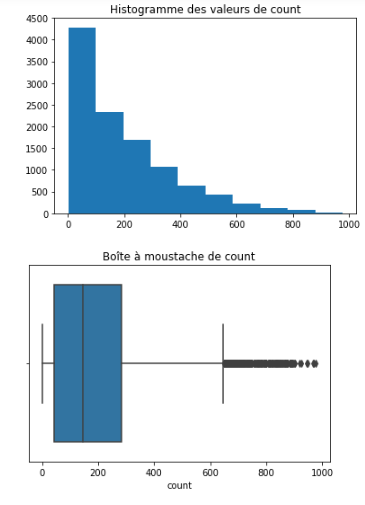
\includegraphics[width=0.5\textwidth]{image_rapport/analyse_count}

Il est donc nécessaire d'effectuer une transformation des données. Ici, nous allons effectuer une transformation logarithmique afin de diminuer l'importance des données trop excentrées par rapport à la moyenne.

\underline{Code pour cela:}

\begin{code-Python}
df_bike_sharing['count']=df_bike_sharing['count'].apply(lambda x:np.log(x))
\end{code-Python}

Maintenant nous allons regarder si il y a une saisonnalité dans les données:
Code:
\begin{code-Python}
df_bike_train['Year'] = pd.DatetimeIndex(df_bike_train["datetime"]).year
df_bike_train['Month'] = pd.DatetimeIndex(df_bike_train["datetime"]).month
x=df_bike_train.groupby(['Year','Month']).sum()
lst=[]
for i in x["count"]:
    lst.append(i) 
\end{code-Python}

\underline{Résultat:}

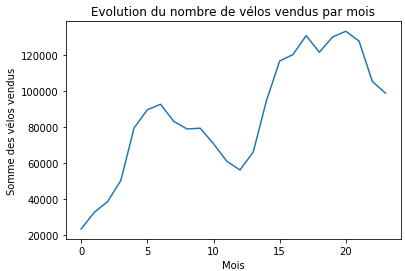
\includegraphics[width=0.5\textwidth]{image_rapport/saisonnalite}

\ On constate bien une forte saisonnalité (il y a beaucoup de locations les mois d'été comparé au mois d'hiver). Mais on constate aussi une forte augmentation des locations d'une année sur l'autre. Il faudra donc supprimer ce phénomène afin d'être plus précis.

Ce phénomène se retrouve dans les températures qui sont par définition un phénomène saisonnier.

Nous allons donc enlever la saisonnalité dans cette variable.

On constate bien ici une saisonnalité annuelle sur les températures:

\underline{Code:}
\begin{code-Python}
df_bike_train["nbr_day"]=1
df_bike_train['Year'] = pd.DatetimeIndex(df_bike_train["datetime"]).year
df_bike_train['Month'] = pd.DatetimeIndex(df_bike_train["datetime"]).month
x=df_bike_train.groupby(['Year','Month']).sum()
lst=[]
for i in x["temp"]:
    lst.append(i)
\end{code-Python} 

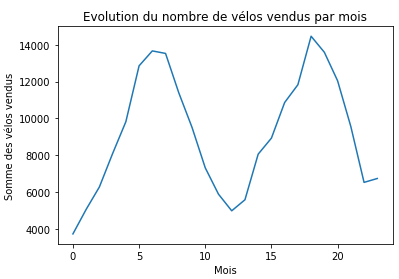
\includegraphics[width=0.5\textwidth]{image_rapport/tempt_fct_mois}

\ Pour éliminer, nous allons nous baser sur un modèle polynomial de Numpy (polyfit).
Ici nous allons estimer nos valeurs avec un modèle polynomiale de type:
$y=x^{6}*b1+x^{5}*b2+x^{4}*b3+x^{3}*b4+x^{2}*b5+x^{1}*b6$
avec ici une équation de degré 6.

\ Ici on retrouve un polynôme de degré pair. Après quelques tests, nous allons prendre un polynôme de degré 6 pour estimer notre modèle.

\underline{Code:}
\begin{code-Python}
from pandas import Series
from matplotlib import pyplot
from numpy import polyfit
series = Series(df_bike_train["temp"])
# fit polynomial: x^2*b1 + x*b2 + ... + bn
X = [i%(365*24) for i in range(0, len(series))]
y = series.values
degree = 6
coef = polyfit(X, y, degree)
print('Coefficients: %s' % coef)
# create curve
curve = list()
for i in range(len(X)):
    value = coef[-1]
    for d in range(degree):
        value += X[i]**(degree-d) * coef[d]
    curve.append(value)
\end{code-Python}

\underline{Résultat:}
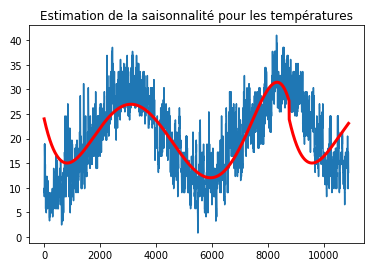
\includegraphics[width=0.5\textwidth]{image_rapport/saison_timeseries}


On va donc utiliser ce modèle pour créer une variable ajustée par rapport à la saisonnalité et remplacer la variable de temps par celle-ci.

\underline{Code:}
\begin{code-Python}
series = Series(df_bike_train["temp"])
# fit polynomial: x^2*b1 + x*b2 + ... + bn
X = [i%(365*24) for i in range(0, len(series))]
y = series.values
degree = 6
coef = polyfit(X, y, degree)
print('Coefficients: %s' % coef)
# create curve
curve = list()
for i in range(len(X)):
	value = coef[-1]
	for d in range(degree):
		value += X[i]**(degree-d) * coef[d]
	curve.append(value)
# create seasonally adjusted
values = series.values
diff = list()
for i in range(len(values)):
	value = values[i] - curve[i]
	diff.append(value)
pyplot.plot(diff)
pyplot.show()
\end{code-Python}

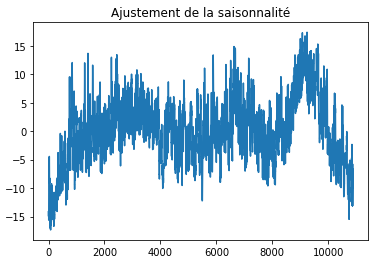
\includegraphics[width=0.5\textwidth]{image_rapport/ajustement_saisonnalite}

On constate tout de même un pic pour l'été 2011.



Nous allons aussi regarder l'évolution des locations en fonction de l'heure de la journée:

\underline{Code:}
\begin{code-Python}
df_bike_train["nbr_day"]=1
df_bike_train['Hour'] = pd.DatetimeIndex(df_bike_train["datetime"]).hour
x=df_bike_train.groupby(['Hour']).sum()
lst=[]
for i in x["count"]:
    lst.append(i)
\end{code-Python}
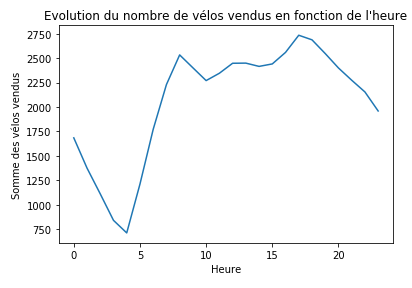
\includegraphics[width=0.5\textwidth]{image_rapport/count_fct_heure}
\newline
Nous pouvons également représenter cette évolution par un diagramme en moustache, en fonction des heures: \newline
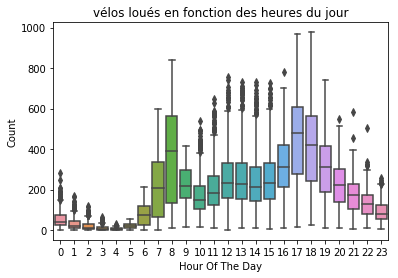
\includegraphics[width=0.5\textwidth]{image_rapport/moustache_count}

On constate de légers pics vers 8h et 17h, cependant pas de très fortes irrégularités pendant la journée; on note en revanche une claire différence entre la journée et la nuit. 
\newline
Observons par ailleurs, s'il est possible de distinguer une tendance selon le statut de l'individu, autrement dit s'il est enregistré ou si ce n'est qu'un usager occasionnel: \newline
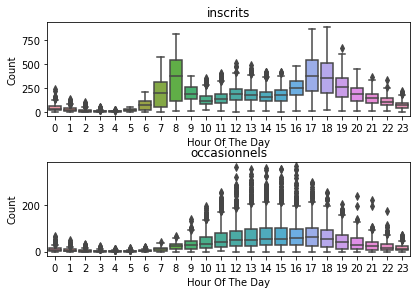
\includegraphics[width=0.5\textwidth]{image_rapport/moustache_registercasual}
\newline
On constate que les utilisateurs occasionnels ont un usage réparti de façon plus uniforme au fil de la journée tandis que les utilisateurs enregistrés ont un usage plus irrégulier se concentrant sur les heures de forte affluence correspondant aux débuts et sorties de travail. \newline


Ainsi, sachant que $registered+casual=count$ avec $count$ notre $target$, on peut envisager de diviser en deux la prédiction avec la partie $registered$ et la partie $casual$ pour obtenir un résultat plus précis avec nos modèles et donc adapter nos $features$ en fonction du statut du locataire. En effet, en plus de la répartition des heures de location qui n'est pas la même, des variables en liaison avec la météo n'auront également pas la même importance selon le statut du l'individu.

\section*{Feature Engineering}
\addcontentsline{toc}{section}{\protect\numberline{}Feature Engineering}%



\qquad Afin de minimiser l'erreur de nos modèles, il est nécessaire de faire un travail préparatoire sur nos données. En effet en rajoutant des $features$, nos modèles seront plus précis (mais évidemment seulement si les $features$ rajoutés sont utiles).

Dans un premier temps, nous pouvons extraire de la date l'heure, le jour, le mois, l'année mais aussi le jour de la semaine.
Ceci est fait avec les lignes suivantes en Python:


\begin{code-Python}
df_bike_sharing['Year'] = pd.DatetimeIndex(df_bike_sharing["datetime"]).year
df_bike_sharing['Month'] = pd.DatetimeIndex(df_bike_sharing["datetime"]).month
df_bike_sharing['Wday'] = pd.DatetimeIndex(df_bike_sharing["datetime"]).weekday
df_bike_sharing['Week'] = pd.DatetimeIndex(df_bike_sharing["datetime"]).week
df_bike_sharing['Day'] = pd.DatetimeIndex(df_bike_sharing["datetime"]).day
df_bike_sharing["Hour"]= pd.DatetimeIndex(df_bike_sharing["datetime"]).hour
\end{code-Python}

\ Ensuite, on remplace les variable $wheater$, $holiday$ et $season$  par des indicatrices. On obtient donc 4 colonnes composées d'indicatrices. Cette méthode permet en effet d'améliorer le modèle.

\underline{Code:}
\begin{code-Python}
df_bike_sharing = pd.get_dummies(df_bike_sharing, columns=['weather'])
df_bike_sharing = pd.get_dummies(df_bike_sharing, columns=['holiday'])
df_bike_sharing = pd.get_dummies(df_bike_sharing, columns=['season'])
\end{code-Python}

\ Ensuite, nous normalisons nos données de température et de température ressentie par une méthode de normalisation $Min-Max$. Elle applique aux données la transformation suivante:
$Data_{ik}^{'}=\frac{Data_{ik}-min(Data_i)}{min(Data_i)-max(Data_i)}\newline$

avec $Data_{ik}^{'}$ la donnée normalisée et $Data_i$ la ième colonne


De plus, comme vu précédemment, nous avons une corrélation entre les variables de température et de météo. Nous allons donc créer une nouvelle colonne qui sera le produit des deux: \newline
\underline{Code:}
\begin{code-Python}
df_bike_sharing['temp_weath_1'] = df_bike_sharing['temp'] * df_bike_sharing['weather_1']
df_bike_sharing['temp_weath_2'] = df_bike_sharing['temp'] * df_bike_sharing['weather_2']
df_bike_sharing['temp_weath_3'] = df_bike_sharing['temp'] * df_bike_sharing['weather_3']
\end{code-Python} 
Par ailleurs, on se basant sur les observations faites plus haut par rapport à la fréquence d'utilisation des personnes enregistrées et des usagers occasionnels, nous avons également créé des variables \verb+daypart+, l'une pour les individus enregistrés \verb+daypart_registered+ et l'autre pour les usagers occasionnels \verb+daypart_casual+. \newline
\underline{Code reprenant l'organisation du découpage des individus enregistrés:}

\begin{code-Python}
   #Pour les individus registered
    df_bike_sharing.loc[(df_bike_sharing['Hour']>=22)  | (df_bike_sharing['Hour']==0),'daypart_registered']=0 #faible affluence
        df_bike_sharing.loc[(df_bike_sharing['Hour']>= 1)  & (df_bike_sharing['Hour']<=5),'daypart_registered']=1 #nuit, tres faible affluence
    df_bike_sharing.loc[(df_bike_sharing['Hour']==6) 
                        | ((df_bike_sharing['Hour']>=10) & (df_bike_sharing['Hour']<=15)) 
                        | (df_bike_sharing['Hour']==20) 
                        | (df_bike_sharing['Hour']==21)
                       ,'daypart_registered']=2 # affluence moyenne
    df_bike_sharing.loc[(df_bike_sharing['Hour']==7),'daypart_registered']=3 #commencement rush
    df_bike_sharing.loc[(df_bike_sharing['Hour']==8),'daypart_registered']=4 #rush
    df_bike_sharing.loc[(df_bike_sharing['Hour']==17)  | (df_bike_sharing['Hour']==18),'daypart_registered']=5 #heures de rush
    df_bike_sharing.loc[(df_bike_sharing['Hour']==9)  
                        |(df_bike_sharing['Hour']==16)  
                        | (df_bike_sharing['Hour']==19)
                        ,'daypart_registered']=6 #affulence importante
\end{code-Python}
\newpage
\underline{Code reprenant l'organisation du découpage des individus occasionnels:}
\begin{code-Python}
    # Pour les occasionnels
    df_bike_sharing.loc[(df_bike_sharing['Hour']>=23)  | (df_bike_sharing['Hour']<=7),'daypart_casual']=0 #nuit, affluence tres faible
    df_bike_sharing.loc[(df_bike_sharing['Hour']== 8) 
                        | (df_bike_sharing['Hour']==9)
                        | (df_bike_sharing['Hour']==21)
                        | (df_bike_sharing['Hour']==22)
                    ,'daypart_casual']=1 #affluence faible
    df_bike_sharing.loc[(df_bike_sharing['Hour']>=10) & (df_bike_sharing['Hour']<=20),'daypart_casual']=2 #affluence plus forte et reguliere sur le jour
\end{code-Python}

A noter que nous utiliserons ces features seulement dans le cas où nous décomposerons la prédiction en deux parties avec deux \verb+target+ : $registered$ et $casual$ tel que $count=registered+casual$.
\newpage
\part{Description des méthodes d'apprentissage automatique utilisées}
\section*{L'algorithme des forêts aléatoires en régression}
\addcontentsline{toc}{section}{\protect\numberline{}L'algorithme des forêts aléatoires en régression}%

\subsection*{Arbre de classification}
\addcontentsline{toc}{subsection}{\protect\numberline{}Arbre de classification}%

\qquad C'est une méthode non paramétrique, qui est assez facilement interprétable car propice à la décision.
L'idée est de construire un arbre binaire de classification. Il est défini par découpages récursifs des régions rectangulaires. On obtient $R_n$ régions qui correspondent aux feuilles de l'arbre. 
La règle en régression est la suivante: 

la moyenne des éléments de l'ensemble $R_i$ auquel appartient notre donnée à prédire est

$y_{n}=\sum_{i=1}^{n}\frac{1}{Card(R_{i})}y_{i}*\mathds{1}_{(x_{i} \in R_{i})} \newline$

\underline{Pour la construction de l'arbre deux questions se posent:}

-comment couper?

-à quelle profondeur s'arrêter?

\qquad En effet, un arbre profond peut sembler bien adapté aux domaines à disposition mais peut être trop complexe (problème de variance). A l'inverse un arbre très peu profond peut être trop grossier et aboutir 
à une régression non concluante.

\qquad On utilise alors l'algorithme $CART$ ($classification$ $and$ $regression$ $trees$) qui choisit à chaque niveau, en commençant par la racine, les variables pour lesquelles le partitionnement a lieu.
A chaque étape, la division choisie est celle qui minimise l'erreur. La stratégie pour la profondeur consiste à construire d'abord un grand arbre puis à l'élaguer de façon à tenir compte du fait qu'une division paraisse plutôt mauvaise à priori mais à une étape suivante peut devenir intéressante.

\subsection*{Bagging (bootstrap aggregating)}
\addcontentsline{toc}{subsection}{\protect\numberline{}Bagging (bootstrap aggregating)}%

\qquad En construisant un arbre de classification ,par essence, la variance est élevée. En effet, chaque division continue à exercer son influence à tous les niveaux suivants et donc une petite perturbation des données entraine une série de divisions assez différentes et donc une régression différente. Il est donc nécessaire de réduire cette variance.

\ La technique du bootstrap est un outil de rééchantillonnage.
Un échantillon bootstrap de taille m des observations initiales est un ensemble de données
$D_{m}=\{(X_{1}^{'},Y_{1}^{'}),...,(X_{m}^{'},Y_{m}^{'})\}\newline$
où les $(X_{i}^{'},Y_{i}^{'})$ sont obtenus par tirage aléatoire uniforme avec remise à partir de 
$D_{m}=\{(X_{1},Y_{1}),...,(X_{m},Y_{m})\}\newline$

Le principe du bagging est une moyenne des prévisions d'arbres de classification sur une collection d'échantillons bootstrap.

Plus précisément, nous prenons B échantillons bootstrap $D_{m}^{b}$ avec $b=1...B$ et on construit un arbre $\hat{f_b}$ associé à chacun.

Pour une nouvelle entrée x, on considère la moyenne des arbres. Pour une régression bagging, on prend la moyenne de chaque échantillon bootstrap soit:

$\hat{f}^{bag}(x)=\frac{1}{B}\sum_{b=1}^{B}\hat{f^{b}}(x)$

\subsection*{Les forêts aléatoires}
\addcontentsline{toc}{subsection}{\protect\numberline{}Les forêts aléatoires}%

\qquad L'algorithme des forêts aléatoires est une version modifiée du bagging avec des arbres moins corrélés.
L'idée est d'améliorer la réduction de variance en réduisant la corrélation entre les arbres. Quand on construit un arbre, on sélectionne aléatoirement un sous-ensemble de $p$ variables parmi les $d$ variables d'entrées qui deviennent candidates pour une division.

\ On va donc ,dans un 1er temps, tirer aléatoirement m-échantillon bootstrap $D_m^b$ à partir de $D_n$.
Ensuite on construit un arbre $\hat{f^b} sur D_m^b$. Cette étape est faite en choisissant $p$ variables parmi $d$ au hasard. Puis on sélectionne la meilleure division parmi ces $p$ variables. Et on itère $B$ fois cette procédure.

\ Enfin on moyenne ces $B$ arbres afin d'obtenir une bonne régression. (Si nous étions dans un problème de classification, on procéderait par vote à la majorité.)

L'inconvénient est une perte d'interprétabilité.


Pour l'implémentation du code, nous avons utilisé la library sklearn.

\underline{Code:}
\begin{code-Python}
import sklearn
from sklearn.ensemble import RandomForestRegressor 
from sklearn import metrics
RFR= RandomForestRegressor()
RFR.fit(X_train,Y_train)
score=cross_val_score(RFR, X, Y, cv=5, scoring='mean_squared_error')
\end{code-Python}

(Nous détaillerons ensuite la partie de cross validation.)

\newpage
\section*{Modèle de mélange et Mélange Gaussien}
\addcontentsline{toc}{section}{\protect\numberline{}Modèle de mélange et Mélange Gaussien}%

\subsection*{Modèle de mélange}
\addcontentsline{toc}{subsection}{\protect\numberline{}Modèle de mélange}%

\qquad A la différence des forêts aléatoires, c'est une méthode paramétrique.
Soit $X_1,...,X_n$ copies indépendantes d'une v.a. $X$ à valeurs dans $\mathbb{R}$ de densité $f$ (qui suit un modèle de mélange fini).

En fait, un modèle de mélange fini de la loi de probabilité consiste à modéliser des données provenant de plusieurs sous-populations. La population totale étant un "mélange" de ces sous-populations.

C'est à la fois un outil de classification/régression mais aussi d'estimation de densité.

Un modèle de mélange s'écrit:
$f(x,\eta)=\sum_{k=1}^{K}p_{k}f_{k}(x)$
où les $f_k $ sont les densités des différentes composantes du mélange.
Les $p_k$ sont les proportions associées (les poids).

Sur les $p_k$, on a:
$p_i >0 $ et $\sum_{k=1}^{K}p_{k}=1$

La loi mélange peut être vu comme la loi marginale de X obtenue à partir de (X,Z) où Z suit une loi multinomiale de paramètres ($1,p_1,...,p_k$) et
X|Z=z suit la loi de densité $f{k:z_{k}=1}$ avec ${z_{1},...,z_{k}}$ un vecteur contenant un 1 et des 0.
Cette interprétation permet de générer un échantillon $X_1,...X_n$ de la loi mélange.   

\subsection*{Mélange gaussien}
\addcontentsline{toc}{subsection}{\protect\numberline{}Mélange Gaussien}%

\ On considère ici que les densités cherchées sont Gaussiennes:
$\ds{f_{k}=\Phi(x,\mu_{k},\Sigma_{k})}$, densité d'une loi gaussienne d-dimensionnelle de moyenne $\mu_{k}$ \newline
et de covariance $\ds{\Sigma_{k}}$.

Ainsi $\ds{f(x,\eta)=\sum_{k=1}^{K}p_{k}\phi\left(x,\mu_{k},\Sigma_{k}\right)}$, avec $\Phi$ densité d'une Gaussienne de moyenne $\mu$ et de covariance $\Sigma$

$\ds{\Phi(x,\mu,\Sigma)=\frac{1}{(2\pi)^{\frac{d}{2}}(\det(\Sigma)^{\frac{1}{2}}} \times \exp\left[\frac{-1}{2}(x-\mu)\Sigma^{-1}(x-\mu)\right]}$

Le vecteur des paramètres est alors:
$\Theta=(p_1,...,p_{k-1},\mu_1,...,\mu_{k},\Sigma_{1},...,\Sigma_{k}$

De plus, $\Sigma_{k}$ est symétrique réelle donc diagonalisable dans une base orthonormée. Elle peut s'écrire $\Sigma_{k}=v_{k}p_{k}D_{k}^{t}p_{k}$ , où $v_{k}=det(\Sigma_{k})^{\frac{1}{d}}$
$D_k$ est la matrice diagonalisable des valeurs propres normalisées de $\Sigma_{k}$ rangées par ordre décroissant avec $det(D_k)=1,$ et $p_k$ est une matrice orthogonale contenant les vecteurs propres de $\Sigma_k$.

Ces éléments permettent de caractériser les propriétés géométriques des composantes:

-le volume est donné par $v_k$

-l'orientation par $p_k$

-la forme par $D_k$ 

Pour se donner un modèle de mélange, il suffit de préciser pour chacune des caractéristiques si elle est supposée identique pour toutes les composantes du mélange ou est autorisée à varier entre les différentes composantes.


Là encore, pour la vise en place de l'algorithme, nous allons utiliser la bibliothèque sklearn:


\begin{code-Python}
from sklearn.mixture import GaussianMixture
GaussianMixture = GaussianMixture()
GaussianMixture .fit(X_train[features],Y_train)
pred = lR.predict(X_test[features])
\end{code-Python}
\newpage
\section*{Les réseaux de neurones}
\addcontentsline{toc}{section}{\protect\numberline{}Les réseaux de neurones}%
\subsection*{Introduction}
\addcontentsline{toc}{subsection}{\protect\numberline{}Introduction}%
\qquad Le modèle de réseau de neurones est un modèle prédictif très en vogue actuellement et qui doit entre autres sa popularité à l'émergence du big data ces dernières années, qui offre des infrastructures permettant d'exploiter leur potentiel. Leur système de fonctionnement s'inspire de celui du cerveau humain (d'où l'origine de leur nom). De façon succincte, ils s'organisent sous forme de couches composées de "neurones" contenant une information que l'on pourra noter $x$. Chacun de ces neurones a une sortie qui va recevoir la somme de plusieurs neurones pondérés par un poids $w$ et auxquelles on va appliquer une fonction d'activation (dont on parlera plus tard) et un biais $w_0$. Si une sortie est connectée par $p$ neurones $x$ de poids $w_p$, une fonction d'activation $a$ et un biais $w_0$, nous avons une valeur de sortie de la forme $\ds{a\left( \sum_{i=1}^{p} w_i x_i + w_0\right)} $ \newline
Il existe plusieurs bibliothèques en Python pour les implémenter dont \verb+tensorflow+ ou bien \verb+pytorch+. Dans le cadre de ce projet, nous utiliserons la bibliothèque  \verb+Keras+ qui est en réalité une "sous-bilbiothèque" de \verb+tensorflow+ et qui permet de créer des modèles de réseaux de neurones intuitivement, efficacement, de façon modulable (et relativement simple).
\subsection*{Vision globale du modèle}
\addcontentsline{toc}{subsection}{\protect\numberline{}Vision globale du modèle}%
Résumé du modèle: \newline
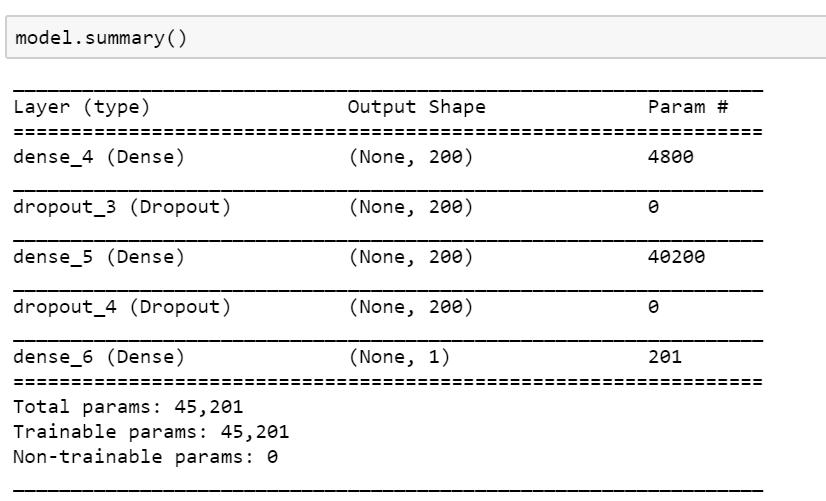
\includegraphics[width=0.8\textwidth]{image_rapport/NNmodelsummary}

\underline{Code d'implémentation du modèle:}
\begin{code-Python}
from keras.models import Sequential

from keras.layers import Dense,Dropout,Activation
from keras import regularizers
# Initialisation du modele

##Define neural network
model = Sequential()
model.add(Dense(200, activation='relu',input_dim=X_trainNN.shape[1])) #input layer
model.add(Dropout(0.1))
model.add(Dense(200, activation='relu')) #hidden layer
model.add(Dropout(0.1))
model.add(Dense(1))#outputlayer
\end{code-Python}

\subsection*{Travail en amont}
\addcontentsline{toc}{subsection}{\protect\numberline{}Travail en amont}%
\qquad Avant d'appliquer un modèle de réseau de neurones, nous avons fait une sélection des $features$ qui seront utiles pour notre modèle prédictif. \newline
Par ailleurs, nous faisons un travail de normalisation sur les données notamment pour les variables continues tel que l'on ait une moyenne nulle et une variance de 1. Cela permet un entrainement plus simple du réseau de neurones et empêche les $features$ avec des valeurs trop importantes d'avoir un impact trop élevé sur le modèle.\newline
Pour la normalisation, nous avons utilisé la méthode du $minimax$ explicitée dans la première partie du rapport. 

\underline{Code pour la normalisation:}
\begin{code-Python}
from sklearn.preprocessing import StandardScaler

# Methode choisie pour normaliser: MinMax
scaler = preprocessing.MinMaxScaler()

# Normalise le train set
X_trainNN = scaler.fit_transform(X_trainNN)

# Normalise le validation set
X_validNN = scaler.fit_transform(X_validNN)

# Normalise le test set
X_testNN = scaler.fit_transform(X_testNN)
\end{code-Python}

\subsection*{Fonction d'activation}
\addcontentsline{toc}{subsection}{\protect\numberline{}Fonction d'activation}%
\qquad Notre modèle de réseau étant un modèle multi-couche qui est le plus adapté dans le cadre de ce challenge. La fonction d'activation la plus régulièrement associée à ces réseaux de neurones et qui donne les résultats les plus intéressants dans notre cas est la fonction \textbf{ReLU} (Rectifier Linear Unit). \newline
\ Cette dernière est particulièrement efficace dans les modèles avec des couches cachées ($hidden$ $layers$) comme ici. Elle s'exprime de la façon suivante: ReLU$(x)=$max$(0,x)$ et permet ainsi de remplacer les valeurs négatives par des 0 (ce qui peut en faire aussi sa faiblesse). Mais elle permet donc de faciliter la convergence du réseau et empécher la saturation.
D'autres fonctions d'activation populaires telles que \textbf{Sigmoid}($\sigma (x) = \ds{\frac{1}{1+e^{-x}}}$) sont parfois plus adaptées mais cette dernière donne un poids important aux petites valeurs et cause la saturation de certains neurones. \newline
\subsection*{Explication du modèle}
\addcontentsline{toc}{subsection}{\protect\numberline{}Explication du modèle}%
\qquad On construit notre modèle sous forme de "pile linéaire de couches" avec \verb+Sequential()+. C'est alors à nous de définir nos couches. Ici, nous avons défini 3 couches: une "input layer", une "hidden layer" et une "output layer" ceci à partir de la fonction \verb+model.add()+ et \verb+Dense()+, ce dernier signifiant que ce sont des couches pleinement interconnectées, avec des inputs de taille 200 dans notre modèle. Cette taille a été déterminée par $"tuning"$, autrement dit en essayant diverses combinaisons de paramètres et regardant celle qui nous donne la plus faible $loss$. La couche finale prenant la valeur 1, représentant le résultat renvoyé. \newline
\ Par ailleurs, nous appliquons un \verb+Dropout+ sur les couches cachées avec un rate de 10\%. Il s'agit d'une technique de régularisation qui consiste à ignorer une certaine proportion de neurones (ici 10\%) durant une session d'entrainement de neurones signifiant que la contribution de ces neurones est temporairement suspendue, ceci permet ainsi d'avoir une prédiction plus généraliste et éviter l'$overfitting$.

\subsection*{Exécution et optimisation}
\addcontentsline{toc}{subsection}{\protect\numberline{}Exécution et optimisation}%
\subsubsection*{Paramètres:} 
\addcontentsline{toc}{subsubsection}{\protect\numberline{}Paramètres}%
\ Le choix du nombre d'époques doit se faire de sorte à avoir une prédiction assez précise et en même temps suffisamment généraliste, c'est-à-dire qui ne $fit$ pas trop les données et provoque de l'$overfitting$. \newline
Le choix de "BATCH\_SIZE" va déterminer le nombre de samples qui vont être propagés à travers le réseau, il va donc influer sur le nombre d'itérations que la machine va faire. Le choix de ce dernier est déterminant pour la vitesse de calcul mais aussi pour la précision de calcul de gradiant.
\begin{code-Python}
# Model parameters
BATCH_SIZE = 16
EPOCHS = 50
LEARNING_RATE = 0.001
\end{code-Python}

\subsubsection*{Optimiseur, métrique et fonction de perte:}
\addcontentsline{toc}{subsubsection}{\protect\numberline{} Optimiseur, métrique et fonction de perte}%
\qquad Avant d'entrainer le modèle, nous utilisons la fonction \verb+compile+ qui va permettre de définir la fonction de perte (ici nous avons choisi la fonction "mse" ou "Mean Squared Error", définie précédemment), un "optimizer" qui va avoir une action sur les poids (définis plus haut) pour minimiser la fonction de perte et une métrique pour mesurer l'erreur du modèle lorsque l'on va entrainer ce dernier après chaque époque. \newline
\qquad Nous avons choisi l'$optimizer$ \underline{"RMSprop"} qui se rapproche beaucoup de \underline{la descente de gradiant}, méthode connue permettant d'optimiser un paramètre (en calculant la pente sur la courbe de perte, et ajustant ce paramètre en fonction du résultat, jusqu'à obtenir un paramètre optimal). \newline
Ce qui le distingue de la descente de gradiant est la façon dont les gradiants sont calculés:

calcul de gradiant avec RMSprop: $\ds{v_{dw}= \beta . v_{dw} + (1 - \beta) . dw}$

calcul de gradiant avec descente de gradiant:$\ds{v_{dw}= \beta . v_{dw} + (1 - \beta) . dw^2}$


Dans notre modèle, l'optimisation des poids était légèrement meilleure avec le calcul de gradiant de RMSprop.\newline
\underline{code python associé:}
\begin{code-Python}
model.compile(loss='mse', optimizer='rmsprop', metrics=['mae'])
\end{code-Python}

\subsubsection*{Entrainement du modèle:}
\addcontentsline{toc}{subsubsection}{\protect\numberline{} Entrainement du modèle}%
\qquad Nous entrainons le modèle avec les paramètres que l'on a définis précédemment. Le réseau de neurones est entrainé en utilisant la \underline{backpropagation} : pour chaque époque, un calcul de perte et d'erreur est fait (définies avec \verb+compile+), voir section suivante pour les résultats. \newline
\underline{Explication brève de la $backpropagation$:}\newline
\ Elle se base sur la décomposition de l'erreur grâce au théorème de dérivation des fonctions, on peut alors écrire la dérivée de l'erreur par rapport au poids de la façon suivante: $\ds{\frac{\partial erreur}{\partial w_{ij}}= \frac{\partial erreur}{\partial f(x)}\frac{\partial f(x)}{\partial z_i}\frac{\partial z_i}{\partial w_{ij}}}$ \newline
\ Avec cette méthode, on a les poids définis plus haut qui sont adaptés après le calcul de gradiant dont on a également parlé précédemment. \newline
A noter que nous entrainons notre modèle sur des données d'entrainement que nous avons splitées.
\begin{code-Python}
history = model.fit(x=X_trainNN, y=Y_trainNN, batch_size=BATCH_SIZE, 
epochs=EPOCHS, verbose=1, validation_data=(X_validNN, Y_validNN), 
                    shuffle=True)
\end{code-Python}


\subsection*{Analyse du modèle et création de prédiction}
\addcontentsline{toc}{subsection}{\protect\numberline{}Analyse du modèle et création de prédiction}%
\subsubsection*{Analyse du modèle:}
\addcontentsline{toc}{subsubsection}{\protect\numberline{} Analyse du modèle}%
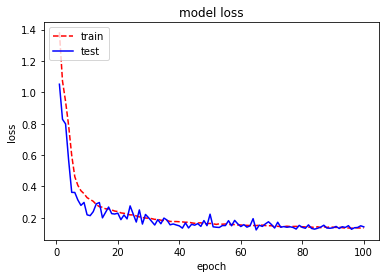
\includegraphics[width=0.8\textwidth]{image_rapport/lossNN} \newline
\ On a bien une convergence de la fonction de perte (ainsi que d'autres fonctions d'erreurs non affichées ici) en fonction du nombre d'époques, ici pour 100 époques, ce qui est un des objectifs (avec aussi le fait d'éviter l'overfitting et l'underfitting).

\subsubsection*{Création de la prédiction:}
\addcontentsline{toc}{subsubsection}{\protect\numberline{}Création de prédiction}%
\ Ci-dessous le code qui nous permet de générer une prédiction a partir du modèle prédéfini par tous les facteurs cités plus haut et entrainé avec ces divers facteurs. Nous appliquons ce modèle au dataset test de kaggle pour soumettre une prédiction par la suite.
\begin{code-Python}
prediction = model.predict(X_testNN, batch_size=BATCH_SIZE, verbose=1)
\end{code-Python}
\newpage
\part{Résultats}
\section*{Outils pour présenter les résultats}
\addcontentsline{toc}{section}{\protect\numberline{}Outils pour présenter les résultats}%

\qquad A la différence des modèles de classification où pour évaluer un modèle on utilise entre autres les matrices de confusion, puis les courbes ROC et l'aire sous cette courbe (l'AUC ou BIC) mais ici ce c'est pas possible. En effet, nous sommes dans un modèle de régression. Nous allons donc mesurer l'erreur.
Nous utiliserons des scores plutôt classiques et la RMSLE utilisée par Kaggle pour évaluer notre modèle:

-l'erreur quadratique moyenne (MSE) $\frac{1}{n}\sum_{i=1}^{n}(y_i-\hat{y_i})^2 \newline$
-l'erreur quadratique moyenne absolue (MAE)  $\frac{1}{n}\sum_{i=1}^{n}\left|y_i-\hat{y_i}\right|^2 \newline$
-l'erreur quadratique moyenne logarithmique (RMSLE) $\frac{1}{n}\sum_{i=1}^{n}(log(y_i+1)-log(\hat{y_i}+1)^2 \newline$

Pourquoi dans notre cas la RMSLE est-elle plus parlante que la MSE ou MAE?

Par exemple, prenons deux exemples:

-le 08/12/2011 à 03:00:00 avec 1 vélo loué

-le 01/08/2012 à 18:00:00 avec 891 vélos loués

\underline{Calculons pour ces deux dates une erreur de prédiction de 10 vélos:}

La MSE sera de 81 et de $(1-11)^2=100$ et de $(891-901)^2=100$ \textbf{ alors qu'il est beaucoup plus grave dans notre cas de prévoir 11 vélos au lieu de 1 plutôt que 901 vélos au lieu de 891.}

La RMSLE permet de régler ce problème.

En effet, $(log(1+1)-log(11+1))^2=0.6$ et $(log(891+1)-log(901+1)^2=1.9*10^-5$

\underline{Code pour la RMSLE:}
\begin{code-Python}
import math
#A function to calculate Root Mean Squared Logarithmic Error (RMSLE)
def rmsle(y, y_pred):
    assert len(y) == len(y_pred)
    terms_to_sum = [(math.log(y_pred[i] + 1) - math.log(y[i] + 1)) ** 2.0 for i,pred in enumerate(y_pred)]
    return (sum(terms_to_sum) * (1.0/len(y))) ** 0.5
\end{code-Python}

\underline{Code pour afficher les différents scores:}
\begin{code-Python}
from sklearn import metrics
print('MAE:', metrics.mean_absolute_error(Y_test, pred))
print('MSE:', metrics.mean_squared_error(Y_test, pred))
print('RMSE:', np.sqrt(metrics.mean_squared_error(Y_test, pred)))
print('RMSE:', np.sqrt(metrics.me(Y_test, pred)))
print('RMSLE:', rmsle(Y_test, pred))
\end{code-Python}
\newpage
\section*{Validation croisée}
\addcontentsline{toc}{section}{\protect\numberline{}Validation croisée}%

\qquad Si on divise nos données seulement en un échantillon d'apprentissage et de test (non utilisé pour l'apprentissage). On calibre l'erreur de la procédure sur notre jeu de données. Donc le calcul d'erreur est d'autant plus précis que l'échantillon de test est grand.

Mais dans la construction de la règle d'apprentissage, nous avons également intérêt à avoir un échantillon assez grand  pour obtenir une règle performante.
Ainsi le découpage échantillon test/apprentissage est intéressant seulement pour un jeu de données très grand (ce que nous n'avons pas ici).

L'idée de la validation croisée est de partager en K échantillons (K-blocs). On va alors donner le statut d'échantillon test à chaque blocs  successivement (les autres devenant les bloc d'apprentissage.
 
$\textbf{Détail de la validation croisée:}$

1ère étape:
Partition aléatoire des données en K sous ensembles $I_1,...,I_k$ (Choix de K par l'utilisateur)

2ème étape:
$\forall k=1,..,K$:
$D_K=\{(X_i,Y_i), i\not\in I_k\}$ (ensemble d'apprentissage)
$D_K=\{(X_i,Y_i), i \in I_{k}\}$=ensemble de validation

Soit $\{\lambda_{i},...\lambda_{d}\}$ un paramètre à calibrer

Pour chaque valeur de $\lambda$, on construit la méthode
$\hat{f_\lambda^{k}}$
Et on calcule l'erreur sur $D_{k}$:

$e_{k}(\lambda)=\sum_{i\in I_{k}}\mathscr{L}(Y_i,\hat{f_{\lambda}^k}(X_i)$ avec $\mathscr{L}$ une fonction d'erreur (voir chapitre ci dessus)

3ème étape:
$\forall \lambda,$ on calcule l'erreur moyenne sur les K-blocs:

$CV(\lambda)=\frac{1}{n}\sum_{k=1}^{K}e_{k}(\lambda)=\frac{1}{n}\sum_{k=1}^{K}\sum_{i\in I_{k}}\mathscr{L}(Y_i,\hat{f_{\lambda}^k}(X_i)$



\underline{Code pour mettre en place une validation croisée:}
\begin{code-Python}
from sklearn.model_selection import cross_val_score
score=cross_val_score(RFR, X, Y, cv=5, scoring='neg_mean_squared_error')
\end{code-Python}


\section*{Score}
\addcontentsline{toc}{section}{\protect\numberline{}Score}%
\qquad Nous avons comparé différents modèles avec les MSE, MAE et surtout RMSLE. Les modèles choisis étaient: Random Forest ,AdaBoost, Machine à vecteur de support, mélange Gaussien et réseau de neurones.

\underline{Code pour obtenir les scores:}
\begin{code-Python}
from sklearn.ensemble import RandomForestRegressor 
from sklearn import metrics
RFR= RandomForestRegressor()
model=RFR
#score=cross_val_score(RFR, X, Y, cv=5, scoring='mean_squared_error')
lst_mse_score.append(format_e(cross_val_score(model, X, Y, cv=5, scoring='neg_mean_squared_error').mean()))
lst_mae_score.append(format_e(cross_val_score(model, X, Y, cv=5, scoring='neg_median_absolute_error').mean()))
lst_rmsle_score.append(format_e(cross_val_score(model, X, Y, cv=5, scoring='neg_mean_squared_log_error').mean()))
\end{code-Python}

\underline{Code pour obtenir les scores des neural networks:}
\begin{code-Python}
from sklearn import metrics
predic= model.predict(X_validNN, batch_size=BATCH_SIZE, verbose=1)
mseNN = metrics.mean_squared_error(Y_validNN, predic)
maeNN = metrics.mean_absolute_error(Y_validNN, predic)
rmsleNN = np.sqrt(metrics.mean_squared_log_error(Y_validNN, predic))
\end{code-Python}

\underline{Code pour affichage du tableau:}
\begin{code-Python}
from prettytable import PrettyTable
t = PrettyTable(['    ','RandomForestRegressor','SVM Regressor','GaussianMixture','AdaBoostRegressor', 'NeuralNetworks']])
t.add_row(lst_mse_score)
t.add_row(lst_mae_score)
t.add_row(lst_rmsle_score)
print(t)
\end{code-Python}


\textbf{Résultats:}

\hspace*{-0.1\textwidth}
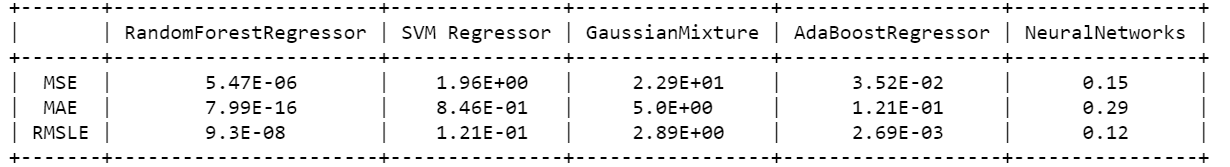
\includegraphics[width=1.2\textwidth]{image_rapport/resultats}

\qquad On constate bien que les Random Forest est l'algorithme qui minimise l'erreur, nous allons donc l'utiliser sur Kaggle.

\section*{Kaggle}
\addcontentsline{toc}{section}{\protect\numberline{}Kaggle}%

\qquad Nous avons ensuite testé nos résultats avec le dataset de test fourni par Kaggle. Celui-ci est un fichier indépendant ne comprenant pas les valeurs pour registered, casual et évidement de count.
Ensuite on enregistre nos prédictions dans un CSV avec les dates et nos prédictions.

\underline{Code pour soumettre sur Kaggle:}
\begin{code-Python}
RFR= RandomForestRegressor()
RFR.fit(X_train[features],Y_train)
pred = RFR.predict(X_test[features])
print(len(pred))
submission = pd.DataFrame({'datetime':df_bike_test['datetime'],'count':pred})
#submission["count"] = submission["count"].astype(int)
#print(submission)
submission["count"]=np.exp(submission["count"])
cpt_row=0
for row_submisson in submission["count"]:
        #print(submission.loc[[cpt_row], ['count']])
    #submission.loc[[cpt_row], ['count']]=submission.loc[[cpt_row], ['count']]
    if row_submisson<0 :
            submission.loc[[cpt_row], ['count']]=0
    cpt_row=cpt_row+1
 
filename = 'Bike Sharing.csv'
submission.to_csv(filename,index=False)
print('Saved file: ' + filename)
\end{code-Python}

Nous avons obtenu une RMSLE au minimum de 
12 days ago by Alexandre Chevaux 0.44763.
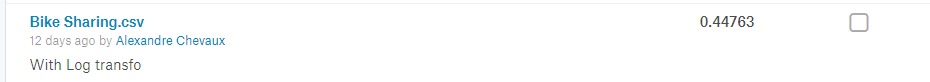
\includegraphics[width=1\textwidth]{image_rapport/Kaggle}

\textbf{Pendant la compétition, cela nous aurait classés à la 844 place sur 3251 soit dans le top 26\%}

Score Kaggle avec réseaux de neurones: \newline
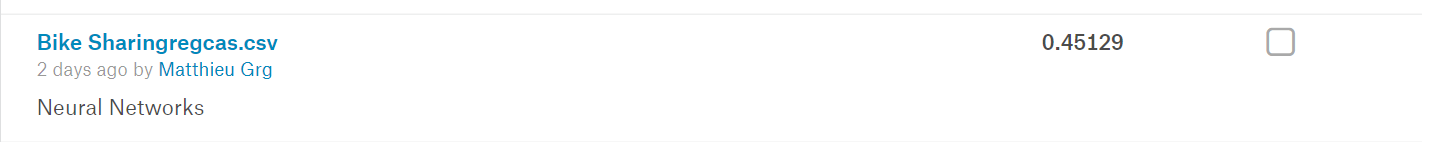
\includegraphics[width=1\textwidth]{image_rapport/scoreNN}
\newpage
\part*{Conclusion}
\addcontentsline{toc}{part}{\protect\numberline{}Conclusion}%

\qquad Ainsi, nous avons traité le sujet Kaggle 'Bike Sharing Demand'. Celui est un sujet de régression qui consiste à prédire le nombre de vélos loués en fonction du jour et de l'heure.
Dans un premier temps, nous avons fait une analyse des différentes variables afin de voir l'intérêt qu'elles présentaient et de les rendre plus pertinentes.

\qquad Ensuite, nous avons effectué un travail sur les données (Feature Engineering). Nous avons par exemple récupéré des informations de la date, groupé certaines informations, effectué une transformation logarithmique de la sortie, enlevé un paramètre de saisonnalité dans la variable de température...

\qquad Trois méthodes d'apprentissage automatique ont ensuite été présentées: les forêts aléatoires, le mélange gaussien et les réseaux de neurones. Cette présentation était à la fois théorique mais nous avons également explicité le code pour les mettre en place.

\qquad Enfin, les méthodes d'évaluation des modèles de régression ont été abordés afin de comprendre les résultats que nous avons obtenus.

\qquad Nous avons obtenu un RMSLE de 0.44763 pour le dataset de test Kaggle ce qui nous classe parmi les 26 premiers pour cent.
  
\newpage
\part*{Bibliographie}
\addcontentsline{toc}{part}{\protect\numberline{}Bibliographie}%

-Cours d'Aurélie Fisher de Data Mining du master ISIFAR (aurelie.fischer-at-univ-paris-diderot.fr)

-https://openclassrooms.com/fr/courses/4297211-evaluez-et-ameliorez-les-performances-dun-modele-de-machine-learning

-https://machinelearningmastery.com/time-series-seasonality-with-python/

- Résumé et idées de travail sur le projet programmé en R: https://www.analyticsvidhya.com/blog/2015/06/solution-kaggle-competition-bike-sharing-demand/

- https://www.datacamp.com/community/tutorials/deep-learning-python

- https://openclassrooms.com/fr/courses/4470406-utilisez-des-modeles-supervises-non-lineaires/4732186-empilez-les-perceptrons

- https://machinelearningmastery.com/


\end{document}